% This is the template for submission of abstracts to NetSci 2017 in Indianapolis, IN.
% It is modified from NetSci 2016.
% The editor of the booklet reserves the right to modify your submission.

%% To process this file run LaTeX2e

%%********DO NOT EDIT****************
\documentclass[12pt]{article}
\usepackage{mathptmx}
\usepackage{graphicx}
\pagestyle{empty}

\setlength\topmargin{0pt}
\addtolength\topmargin{-\headheight}
\addtolength\topmargin{-\headsep}
\setlength\oddsidemargin{0pt}
\setlength\textwidth{\paperwidth}
\addtolength\textwidth{-2in}
\setlength\textheight{\paperheight}
\addtolength\textheight{-2in}
\usepackage{layout}

\renewcommand{\title}[1]{\noindent\textbf{#1}\bigskip\\}
\renewcommand{\author}[1]{\noindent #1\bigskip\\}
%%***********************************

\begin{document}

%**********USER DEFINED**************
%Enter title here
\title{Towards Attack-Tolerant Networks: Multipath Fault Tolerance}
%Enter author(s) and address here
\author{Edward L. Platt$^1$ and Daniel M. Romero$^1$\bigskip\\
{\small
1. University of Michigan, Ann Arbor, MI, USA\\
}
}
%Enter abstract here
Centralized systems are susceptible to
targeted attacks against central points,
suggesting the importance of decentralization in attack-tolerant systems.
While many techniques exist for tolerating random faults,
better techniques for tolerating {\em adversarial faults} such as targeted attacks are needed.
In communication networks, targeted attack can leave users vulnerable to
censorship and surveillance of messages at central points.
Even when encryption is used, it can be bypassed by coercion, e.g., subpoenas.
While decentralized {\em protocols} have become a popular approach to attack-tolerance, centralized network {\em
structure} can arise even when protocols are
decentralized.
Despite their decentralized protocols,
the internet and World-Wide Web have
been shown both theoretically and historically to be highly susceptible to
adversarial faults [1], in part due to emergent structural centralization.
In this work, we present
1. A fault tolerace scheme for networked communication having a failure probability that decreses exponentially with the number of available independent paths;
2. A routing algorithm for constructing such indpendent paths in the butterfly network topology [2]; and
3. A bounded-transitivity trust model that makes it possible to quantify the adversarial fault tolerance of a network.
Our work is the first theoretical demonstration of a point-to-point communication network architecture able to tolerate coercion and other
targeted attacks, without requiring infinitely transitive trust.
We also evaluate the fault tolerance of an imperfectly implemented butterfly topology by partially rewiring a snapshot of the internet's router network.
We find that rewiring only 10\% of the edges allows the network to withstand faults in the most central 2\% of nodes,
increasing to 8\% of nodes for 90\% rewiring.
Our results show that it is possible, in principle, to create highly attack-tolerant communication systems that can withstand targeted and coercive attacks, but only when it is possible to influence network structure.
\begin{figure}[!h]
\begin{center}
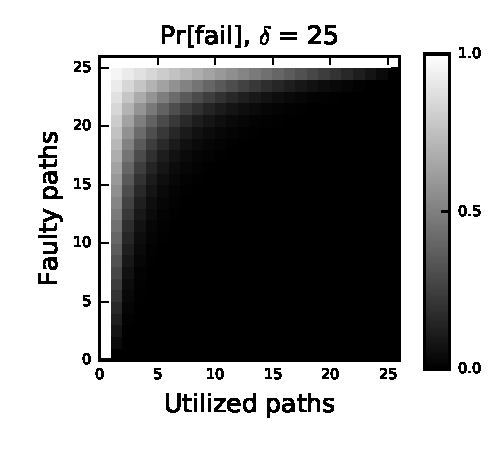
\includegraphics[scale=0.75]{fig-perror}
\end{center}
\caption{
Failure probability decreases rapidly with the number of
message copies, and increases slowly with the number of faults.
Messages are difficult to attack and easy to defend.
}
\end{figure}

\noindent[1] R. Albert et al. Error and attack tolerance of complex networks. {\em Nature,} 406(6794), 2000.
\\
\noindent[2] A. D. Kshemkalyani and M. Singhal. {\em Distributed Computing}. Cambridge U. Press, 2008.


% Place the abstract of your talk/poster here, 250 Words maximum.
% Mathematical formulae may be set in LaTeX, but do NOT use the
% bibliography environment -- if you must have references, use an 
% enumerated list.
%
% Your abstract (plus one figure) should not exceed one page.
%
% Check carefully.

%************************************
\end{document}